\documentclass[sigconf,natbib=false]{acmart}
\settopmatter{printacmref=false}

\usepackage[style=ACM-Reference-Format,backend=bibtex,sorting=none]{biblatex}
\addbibresource{base.bib}

\usepackage[lofdepth,lotdepth]{subfig}

\emergencystretch=1em

%% remove copyright and further ACM refs for the Lab
\setcopyright{none}
\copyrightyear{2021/2022}
\acmDOI{}
\acmISBN{}
\acmConference[Data Science Lab]{Data Science Lab}{2021/2022}{Uni Passau}

%% end of the preamble, start of the body of the document source.
\begin{document}

%%
%% The "title" command has an optional parameter,
%% allowing the author to define a "short title" to be used in page headers.
\title{Data Augmentation for Improved Morphology on Mars Data}

%% author list and team
\author{Douglas D. Agbeve}
\email{agbeve01@ads.uni-passau.de}
\affiliation{\institution{University of Passau}}
  
\author{Aditya V. Handrale}
\email{handra01@ads.uni-passau.de}
\affiliation{\institution{University of Passau}}
  
\author{Salim Fares}
\email{fares01@ads.uni-passau.de}
\affiliation{\institution{University of Passau}}
  
\author{Seif E. Idani}
\email{idani01@ads.uni-passau.de }
\affiliation{\institution{University of Passau}}

\renewcommand{\shortauthors}{Team 5}

%%
%% The abstract is a short summary of the work to be presented in the
%% article.
%\begin{abstract}
%A generally good scheme for an abstract is the following:
%\begin{itemize}
 %\item The problem?
 %\item Our solution.
 %\item Our solution in detail.
 %\item So what?
%\end{itemize}
%(1-2 sentences each). 
%You don't need to provide an abstract during the first 3 phases, as you most likely will not have an answer to all items.
%It should be included in your phase 4 submission and the final document.
%\end{abstract}


%%
%% This command processes the author and affiliation and title
%% information and builds the first part of the formatted document.
\maketitle
\section{Introduction}
A picture, they say, is worth a thousand words. As a medium of communication,
pictures have been used since the dawn of \textit{Homo Sapiens}\cite{Yuval},
which makes understanding the information embed in them a major part of research
in the various fields of science ranging from Archaeology to the relatively
more recent Computer Science.\par
In Computer Vision, a vital process in retrieving information in images and
which form part of most systems for visual understanding is image
segmentation\cite{ForsythPonce}. It is the process of partitioning an image or a
video frame into multiple segments\cite{YingTan}. Segments are fundamentally a
set of pixels in a region that share a common property such as colour or
texture, enabling the identification and locating of boundaries of objects in an
image\cite{DassDevi}. Digital image segmentation is applied in various domains, 
including but not limited to, medical (locating cancerous tumors and measuring
tissue volumes)\cite{PhamXuPrince}, facial and fingerprint recognition,
self-driving vehicles (detecting pedestrian). There are and continue to be
proposed, many algorithms for image segmentation. Currently, these approaches are
either segregating pixels based on intensity changes (i.e.~detecting discontinuity)
such as edge detecting algorithms, or partitioning an image into regions with
similar predefined criteria (i.e.Similarity detection) examples include
thresholding approaches. The various algorithms can also be categorized based on
the method used in solving the problem; namely (1) Edge detection based
segmentation e.g.~histogram-based\cite{ZengLiMengYangLiu} and
gradient-based\cite{SaifHammadAlqubati}, (2) Thresholding approaches such
as those proposed by Abd Elaziz \textit{et al}\cite{ElazizBhattacharyyaLu}, and
Houssein \textit{et al}\cite{HousseinEmamAli}, (3) Region-based segmentation
techniques include region growing\cite{ChengWang, Jothiaruna}, region split and
merge\cite{Lachaize, LiuSclaroff}, (4) techniques based on Partial Differential
Equation are active contour\cite{KassWT}, C-V model\cite{WangWWF} etc., (5)
Clustering methods such as K-means clustering algorithm\cite{YanCaiGaoLuo} and
relatively more recent approach is the Artificial Neural Network (ANN) algorithms
which solves image segmentation problems with higher accuracy compared to other
approaches. Examples of Deep learning or ANN approach to image segmentation
include but not limited to Convolutional Network models such as VGG16,
GoogLeNet, Fast R-CNN, Faster R-CNN\cite{ren2016faster},
U-NET\cite{ronneberger2015unet}, V-NET\cite{milletari2016vnet} and
Mask-RCNN\cite{he2018mask}, Recurrent Neural Network models include
ReSeg\cite{visin2016reseg},Generative and Adversarial (GAN) Models e.g.
\@\cite{luc2016semantic, 8237868,hung2018adversarial}, a comprehensive list of
GAN-based techniques can be found at~\cite{ganzoo}.
\par
The problem of image segmentation can be coined as that of classifying pixels
with semantic labels i.e.~semantic segmentation (fig.~\ref{fig:SSeg}) or
segregating pixels into individual objects in the image i.e.~instance
segmentation (fig~\ref{fig:ISeg})\cite{PaneruJeelani}. In semantic segmentation,
pixels are assigned to the same segment if they are of the same object type in
the image. This can be thought of as classification at pixel level. Instance
segmentation involves assigning all the pixels that belong to the same single
object to the same segment. It is a two-step process; extracting bounding
boxes around each instance of an object through object detection and then
classifying pixels that  corresponding to each instance in the bounding box.
This technique combines object detection (fig.~\ref{fig:ObjDet}) and
segmentation. A third, relatively new, formulation is to combine both instance
and semantic segmentation termed Panoramic Segmentation (fig.~\ref{fig:PSeg}).
It involves the detection and segmentation of all objects including background
and labelling different instances in an image.\par
Digital Elevation Models (DEMs) are essential in analyzing erosion and drainage,
hill-slope hydrology, studying groundwater flow, watersheds, and contaminant
transportation as they are important tools for parameterizing topography. DEM is
representation of planetary (earth, moon, mars etc.) terrain from elevation data
in 3-D image. There are two types; raster Geographic Information Systems (GIS)
layer representation and the vector-based triangular irregular network format.
DEMs are obtained using techniques such as Surveying, Stereo Photogrammetry,
Lidar, Radar, etc.. Flight and Train simulations, GIS and Satellite navigations
are some of the systems in which DEMs are used. Martian surface has an abundance
of geographical features such as volcanoes, layers and gullies, with phenomena
like volcanoes bringing out microbial entities that were protected from solar
radiation. Moreover, glaciers and mounds that have water underneath them might
contain evidence of life. Detecting and studying these morphologies can help us
find extraterrestrial life on mars. The detection of mounds formed from
phenomena such as volcanic eruption can be done automatically using ANN based
image segmentation methods.
\begin{figure}[ht]
    \centering
    \subfloat[input image][Input Image]{
        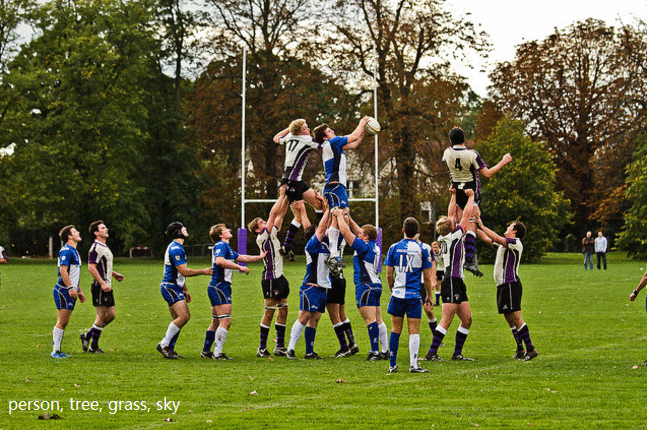
\includegraphics[width=0.225\textwidth]{images/input_image.png}\label{fig:inputImage}
    }
    \subfloat[object detection][Object Detection]{
        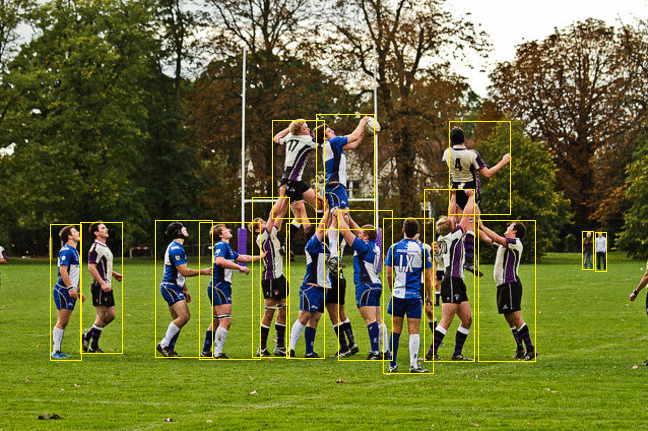
\includegraphics[width=0.225\textwidth]{images/object_detection_image.png}\label{fig:ObjDet}
    }
    \newline
    \subfloat[semantic image][Semantic Segmentation]{
        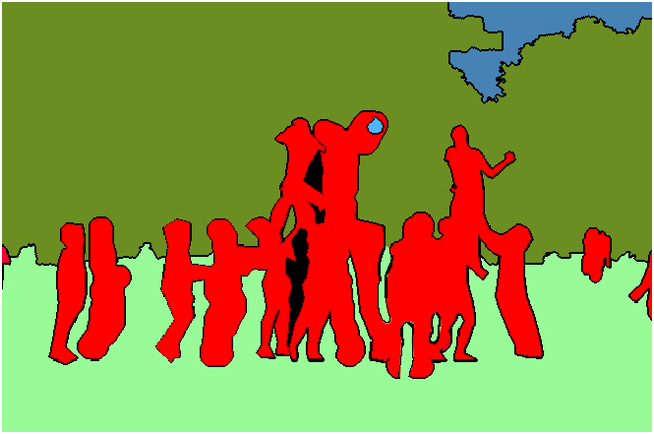
\includegraphics[width=0.225\textwidth]{images/semantic_image.png}\label{fig:SSeg}
    }
    \subfloat[instance image][Instance Segmentation]{
        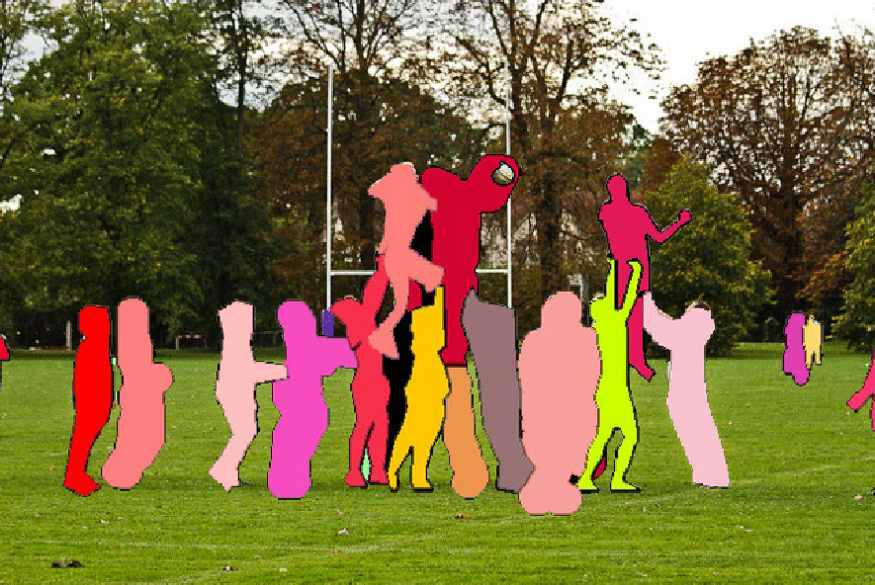
\includegraphics[width=0.225\textwidth]{images/instance_image.png}\label{fig:ISeg}
    }
    \newline
    \subfloat[panoramic image][Panoramic Segmentation]{
        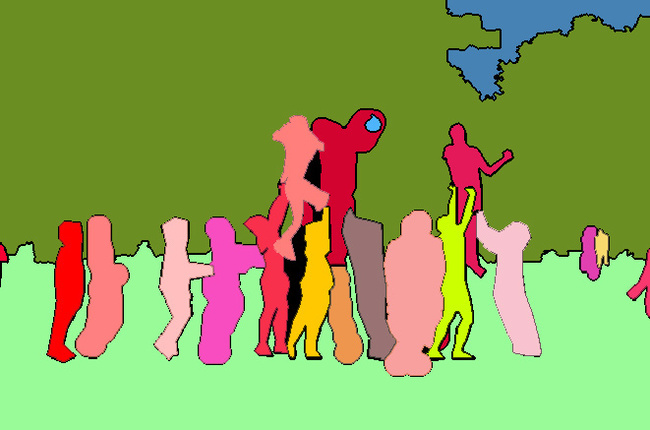
\includegraphics[width=0.3\textwidth]{images/panoramic_image.png}\label{fig:PSeg}
    }

    \caption{Variations of Segmentation~\cite{BigdataAILab}}
\end{figure}
\subsection{Research Questions}
The many algorithms available for solving image segmentation problem is an
indication that no single approach can solve it all accurately and in a more
efficient way. An affirmation of this assertion is the numerous methodologies
proposed in literature by Deep Learning researchers in recent decade.
Furthermore, the choice of algorithm and by extension the need for new
approaches, is principally influenced by data pertaining to the problem, its
representation and the type of segmentation problem.
In view of these, we formulated the following questions with regard to the data
at hand.
\begin{itemize}
    \item Will data augmentation have any effect on the accuracy of our selected
        approach (es) for application, and if yes, how much extra data relative
        to the training data?
    \item Which of the Machine Learning, more specifically Deep learning,
        techniques, segments the data with much more accuracy?
    \item Most of the Deep Learning algorithms in literature are categorize
        under supervised learning. Can this problem be solved with unsupervised
        learning techniques?
\end{itemize}
\subsection{Related Work}
Wuff-Jensen \textit{et al.} proposed, to the best of our knowledge, the original
idea of using GANs to generate terrain from DEMs. Their architecture was based
on deep convolutional GAN (DCGAN)\cite{RMC}~--~a type of GAN made up of a
fractional-strided convolutions (generator) and a discriminator of strided
convolutions.\par
Spick \textit{et al.}\cite{SpickCW} presented a method of generating height maps
from digital elevation of regions of earth. The authors approach was based on
Spatial GANs (SGAN)\cite{JetchevBV}. Spatial GANs remove fully connected layers
from DCGAN allowing outputs to be scaled to any size and mapping features onto
output as translation-invariant.\par
Bowles \textit{et al.}\cite{bowles2018gan} investigated augmenting training data
using GAN-derived synthetic images. Progressive Growing of GANs
(PGGAN)\cite{KarrasAJ} network was used as a baseline architecture, and
demonstrated that this can improve results across two segmentation tasks
(1)~-~Computed Tomography (CT) images with manually delineated Cerebrospinal
Fluid (CSF) labels, (2)~-~Fluid-Attenuated Inversion Recovery (FLAIR) images
with manual White Matter Hyperintensity (WMH) segmentations.
\section{Problem statement}
In this section, we formally present the problem of automatically detecting
mounds in Mars' Arabia Terra. Specifically, classification of pixels in the
digital elevation model of Mars in to segments of mounds or no-mounds using
using Artificial Neural Network based techniques. We sought to predict where
mounds given any DEM of Mars\par
More formally, given $n$ annotated images $\lbrace x_{1},x_{2},\ldots,x_{n}
\rbrace$ and each image, say $x_{i}$, has $m_{i}$ objects that are categorize
into $C$ classes with objects labelled as $y_{i}$.
\begin{equation}
    y^{i} = \lbrace (c^{i}_{1},v^{i}_{1}), (c^{i}_{2},v^{i}_{2}, \ldots,
    (c^{i}_{m_{i}},v^{i}_{m_{i}})) \rbrace
\end{equation}
\hspace{2em} {$where$} $c^{i}_{m_{i}}\in C$ and $v^{i}_{m_{i}}$ is the object's
pixel mask.\\
The goal is to learn the values of some parameterized $(\theta)$ function $f$
such that:
\begin{equation}
    y^{i} = f(x_{i},\theta_{i})
\end{equation}
And be able to predict object (mound) locations $\hat{y}$ for all new (unseen)
$x_{i}$\\
A loss function to optimize the prediction would be:
\begin{equation}
    J(\theta) = \dfrac{1}{n}\sum_{i=1}^{n}l(\hat{y}^{i},x_{i},y^{i};\theta) +
    \dfrac{\lambda}{2}\| \theta \|^{2}_{2}
\end{equation}
Due to the relatively small number of training samples, we proposed, as a
starting point of our implementation, inspired by the work done by Souly
\textit{et al.}\cite{8237868}, an architecture with a generator to provide extra
training samples and classifier as a discriminator in a Generative Adversarial
Network. We evaluate the performance of each approach against the following
metrics \textit{Pixels Accuracy} i.e.~ratio of properly classified pixels to
total number of pixels, \textit{Mean Pixel Accuracy (MPA)} is the average of the
ratio of properly classified pixels to the number of pixels in a class and
\textit{Mean Intersection over Union (mIoU)} is the ratio of the intersection
between the ground truth and the predicted segmentation map to their union,
averaged over all classes.
\printbibliography{}

\appendix
\section{Phase Contribution}
\begin{itemize}
    \item Phase One \hspace{2em} Douglas D. Agbeve 
\end{itemize}
\end{document}
